\section{Evaluation}\label{s:eval}

We have seen in Figure~\ref{fig:design:shift-bottleneck:after} that \name can move the network queues to the \inbox to gain control over scheduling. 
We now evaluate the following aspects of our design.
\begin{enumerate}
    \item Where do \name's performance benefits come from? We discuss this in the context of improving the flow completion times of \name's component flows. (\S\ref{s:eval:fct})
    \item Can \name enforce different scheduling policies? (\S\ref{s:eval:policies})
    \item Under what conditions do \name's performance benefits hold? (\S\ref{s:robust:cross})
\end{enumerate}

\subsection{Understanding Benefits}\label{s:eval:fct}

\paragrapha{Experimental Setup}
We evaluate our implementation of \name (discussed in \S\ref{s:impl}) using network emulation via mahimahi~\cite{mahimahi}.
Mahimahi creates a Linux network namespace and applies some network condition (emulated delay or link bandwidth) to all packets that traverse it.

There are three $8$-core machines in our setup: one machine is a sender, another is configured as a middlebox and runs an \inbox, and a third is the receiver. Throughout our experiments, CPU utilization on the machines remained below $10$\%.
It is important for experiment fidelity to run the sending application on a different machine than the \inbox; otherwise, because the \inbox data-path uses tc (\S\ref{s:impl}), TCP small queues (TSQ) unrealistically avoids queueing.
The \outbox runs on the same machine as the receiver, inside the same mahimahi network namespace as the receiving application.
\an{somebody make sure this makes sense}\an{Since our prototype implementation uses the Linux kernel datapath, we disable TCP segmentation offload (TSO) and generic receive offload (GRO) on the machines to maintain a consistent view of packet headers between the \inbox and the \outbox.
This is an artifact of our prototype implementation of the \outbox using \texttt{libpcap}: in a real deployment, the \outbox would have the same view of the packets as the \inbox.}

The application we use emulates web traffic: a many-threaded client generates requests from a given empirical request size CDF~\cite{caida-dataset} and assigns them to one of $200$ server processes on the traffic generator.
Each server then sends the requested amount of data to the client and
we measure the flow completion time of each such request.
We use multiple server processes to emulate multiple machines behind the \name at the customer's edge.

Each CDF shown in this section is comprised of $100,000$ requests sampled from this distribution, across $10$ runs each with a different random seed.
In addition, there is a persistently backlogged connection inside the traffic aggregate that models a background large data transfer which would normally fill the bottleneck queue.
%
\cut{
\radhika{Another way to structure the the rest of this section: /*}
\begin{itemize}
    \item Subsection: ``Understanding \name's performance benefits''. 
    \begin{itemize}
        \item (This will cover most of what you have under ``Flow Completion Time'')
        \item Experiment setup (what you currently have)
        \item Result: (Figure~\ref{fig:eval:best})
        \item Explaining why
        \begin{itemize}
            \item Effective bottleneck shifting: a graph that shows queuing delay at mahimahi without bundler, and graphs that show the queuing delay at mahimahi and inbox when using bundler. \an{(this is figure~\ref{fig:design:shift-bottleneck}, should we repeat it?)}
            \item Scheduling is necessary: comparison with FIFO -- what you have now
        \end{itemize}
        \item Comparison with ideal case: mahimahi link does sfq. Show we are not too bad (is it possible to get this result?). \an{will try, but it may not be possible to run sfq in mahimahi}
    \end{itemize}
    \item Subsection: ``Using \name to enforce different policies''.
    
    \begin{itemize}
        \item We use same set-up as before, but different scheduling and queue management polcies at the \name to meet different requirements. 
        \item Improved FCTs using FQ: Helps short flows achieve a smaller FCT by reducing the queuing delay that they see. Results already shown in previous subsection. 
        \item Smaller Queuing Delay using AQM: Helps keep queuing delay small. Present another FCT graph like Figure~\ref{fig:eval:best}, but with FQ-CoDel or PI. Also present a graph which shows the CDF of per-packet delays (if possible). Also, if possible (and if space), a comparison with properly configured and badly configured AQM scheme in the mahimahi link.
        \item Improved Rate Stability 
        \item Prioritizing interactive traffic
        \item anything else? 
    \end{itemize}
    \item Subsection: Robustness analysis
    \begin{itemize}
        \item We vary different aspects of the experiment setup detailed earlier to see how they impact our key results. We use SFQ as the scheduling policy in the bundler, but similar trends would hold for other policies (?). 
        \item Impact of congestion control (what you have now) [might also be fine if it goes in the previous subsection]
        \item Impact of offered load (what you have now)
        \item Impact of path characteristics
        \item Alternative design choices (TCP Proxy)
        \item Impact of cross traffic
        \begin{itemize}
            \item Cross traffic in it's own bundle
            \item Cross traffic not using bundle
        \end{itemize}
    \end{itemize}
\end{itemize}
\radhika{*/}
}
%
%\radhika{another title for this section, or some preceding explanation on what each section is about}
%
%\cut{Note that it is important to use many server processes so that the effect of head-of-line blocking on the client requests is limited.
%Indeed, all the CDFs presented in this section have a ``knee'' where the effects of head-of-line blocking become apparent.
%}
%\radhika{when the graphs are presented, explain the `knee' as an artifact of our expts caused due to some HoL blocking. Btw, are you sure that's why you have the knee?}

\begin{figure}
    \centering
\begin{knitrout}
\definecolor{shadecolor}{rgb}{0.969, 0.969, 0.969}\color{fgcolor}
\includegraphics[width=\maxwidth]{figure/eval:best-1} 

\end{knitrout}
    \caption{\name achieves 33\% lower median slowdown. Note the differing axis scales. For both \name and Optimal, performance benefits come from preventing short flows from queueing behind long ones.}
    \label{fig:eval:best}
\end{figure}
\newcommand{\overviewBenefitsBaselineMedian}{1.62\xspace}
\newcommand{\overviewBenefitsBaselineTail}{10.77\xspace}
\newcommand{\overviewBenefitsBundlerMedian}{1.08\xspace}
\newcommand{\overviewBenefitsBundlerTail}{9.84\xspace}
\newcommand{\overviewBenefitsOptimalMedian}{1.08\xspace}
\newcommand{\overviewBenefitsOptimalTail}{4.46\xspace}
\newcommand{\overviewBenefitsBundlerMedianImprovement}{33\%\xspace}

\an{"Baseline" -> "Status Quo"}
\an{"Optimal" -> "In-Network"}
\paragrapha{Comparison with Optimal and Baseline} 
We first present results for a simplified scenario without any cross-traffic, i.e. all traffic traversing through the network is generated by the same customer and is, therefore, part of the same bundle. 
This scenario highlights the benefits of using \name when the congestion on the bottleneck link in the network is self-inflicted by a single customer. We explore the effects of queues at the bottleneck caused by other cross-traffic in \S\ref{s:robust:cross}.

On a $96$Mbps link, we generate $84$Mbps of offered request load from a CDF with a heavy-tailed request size CDF drawn from an Internet core router~\cite{caida-dataset}.
The workload is heavy-tailed: 97.6\% of requests are 10KB or shorter, and the largest 0.002\% of requests are between $5$MB and $100$MB.

We evaluate three configurations. 
The ``Baseline'' configuration represents the status quo: the \inbox simply forwards packets as it receives them, and the mahimahi bottleneck uses FIFO scheduling.
The ``Optimal'' configuration deploys fair queueing\footnote{
We implement this scheme by modifying mahimahi (our patch comprises $171$ lines of C++) to add a packet-level fair-queueing scheduler to the bottleneck link.}
at the mahimahi bottleneck. 
Recall from \S\ref{s:intro} that this configuration is not deployable in practice: it would force all customers --- who may desire diverging scheduling policies --- to use the same scheduler.
Finally, for the \name configuration, we use a Copa~\cite{copa} congestion controller at the \inbox to manage the bottleneck queue, and the stochastic fair queueing~\cite{sfq} scheduling policy. 

Figure~\ref{fig:eval:best} presents the results with the above experiment setup.
With \name, the median 
slowdown\footnote{We define the ``slowdown'' of a request as its completion time divided by what its completion time would have been in an unloaded network. A slowdown of $1$ is optimal, and lower numbers represent better performance.} 
decreases from $1.62$ for Baseline to $1.08$ with \name: 33\% lower.

Furthermore, \name's performance is near to the benefits that could be achieved with Optimal.
Both \name and Optimal achieve an identical median slowdown of $1.08$.
Optimal provides better performance in the tail: the $99\%$ile slowdown is $4.46$ for ``optimal'' and $9.83$ for \name.
Note that the baseline achieves a $99\%$ile slowdown of $10.77$.
We next discuss the source of this higher tail FCT compared to Optimal.

\paragrapha{Necessity of scheduling} \an{move this text to earlier?}It is important to note that \name by itself is not necessarily a means of achieving low end-to-end delays, as promised by recent efforts in congestion control~\cite{copa, nimbus}, despite its use of these modern congestion control algorithms.

To see why this is the case, recall that \name does not modify the end-hosts: they continue to run the default Cubic congestion controller, which will probe for bandwidth until it observes loss.
Indeed, the packets end-host Cubic sends beyond those the link can transmit must queue somewhere in the network or be lost. Without \name, they get queued up at the bottleneck link.
With \name, they instead queue at the \inbox.
However, the congestion controller at \inbox must also additionally maintain some standing queue at the bottleneck link to make decisions effectively.
Therefore, we expect the overall end-to-end-delays to increase slightly.
As a result, \emph{solely} using a more sophisticated congestion control algorithm at the \name is unlikely to be the cause of significant reductions in the flow completion time.

This is why the tail FCT for \name does not match Optimal's.
We can see this by measuring the relative performance of using FIFO scheduling at the \name instead of the SFQ scheduling in Figure~\ref{fig:eval:best}.
The results are in Figure~\ref{fig:eval:fifo}. 
Unsurprisingly, the FCTs with FIFO scheduling at \name are \emph{worse}: with a median FCT of $173$ms, it is $18$\% higher than the baseline. 
\begin{figure}
    \centering
\begin{knitrout}
\definecolor{shadecolor}{rgb}{0.969, 0.969, 0.969}\color{fgcolor}
\includegraphics[width=\maxwidth]{figure/eval:fifo-1} 

\end{knitrout}
    \caption{With FIFO scheduling, the benefits of \name are lost: FCTs are 18\% worse in the median.}
    \label{fig:eval:fifo}
\end{figure}
\newcommand{\overviewBenefitsFifoMedian}{1.96\xspace}
\newcommand{\overviewBenefitsFifoWorse}{18\%\xspace}


\subsection{Different Scheduling Policies}\label{s:eval:policies}

\begin{figure}
    \centering
\begin{knitrout}
\definecolor{shadecolor}{rgb}{0.969, 0.969, 0.969}\color{fgcolor}
\includegraphics[width=\maxwidth]{figure/eval:lowdelays-1} 

\end{knitrout}
    \caption{We configure \name with the fq-codel scheduling policy to achieve low end-to-end queueing delays.}
    \label{fig:eval:lowdelays}
\end{figure}

\paragrapha{Achieving Low Delays}
\name can configure its scheduling policy to achieve low end-to-end-delays.
In Figure~\ref{fig:eval:lowdelays}, we show that when we configure the scheduling policy at \inbox, we can change the RTTs component connections observe.
Note that due to the effect discussed above, using FIFO scheduling results in higher delays than the baseline case.

\paragrapha{Rate Stability}\label{s:eval:ratestable}

\begin{outline}
    \1 \name can improve the rate stability of component traffic
    \1 One such class of traffic is video streaming
\end{outline}

\paragrapha{Strict Priorities}

\begin{outline}
    \1 \name can support strict priorities for interactive traffic.
    \1 Experiment: backlogged iperf flows are in a lower priority queue and interactive ETG flows are in a high priority queue.
\end{outline}

%\radhika{need to further clean this.}

\subsection{Terminating TCP Connections}\label{s:eval:proxy}
An alternate implementation choice for a \name would use a TCP proxy to terminate connections at the \inbox. 
%\radhika{I assume we mention this in an earlier section? else we need a line or two about why this experiment is interesting.}
We consider the best-case outcome of terminating TCP connections --- the effective RTT observed by the end-to-end congestion controller running at the servers would decrease (since the proxy would acknowledge its segments much faster than the original receiver would), and it would grow its window rapidly.
A proxy-based design would then apply scheduling policy to component traffic (recall that we use SFQ).
We emulate this best-case scenario by modifying the end-hosts to maintain a constant congestion window of $450$ packets --- slightly larger than the BDP --- and increasing the queue lengths at the \inbox to hold these packets. The other aspects of \name remain unchanged.
The result is in Figure~\ref{fig:eval:proxy}.
%
\begin{figure}
    \centering
\begin{knitrout}
\definecolor{shadecolor}{rgb}{0.969, 0.969, 0.969}\color{fgcolor}
\includegraphics[width=\maxwidth]{figure/eval:proxy-1} 

\end{knitrout}
    \caption{A proxy-based implementation of \name could yield further benefits to the long flows. Note the different y-axis scales for each group of request sizes.}
    \label{fig:eval:proxy}
\end{figure}

%
\an{check this text}
For the short requests, terminating TCP connections does not yield additional benefits: with or without termination, they finish in a few RTTs and never leave slow start.
For medium-to-long requests, terminating TCP connections yields benefits since they no longer incur the penalty of window growth.

\subsection{Impact of Congestion Control} \label{s:robust:cross}\label{s:eval:cc}
How does our choice of congestion control impact our results? 
We first verify that \name indeed runs congestion control algorithms appropriately.
\begin{figure}
    \centering
    \begin{subfigure}[b]{0.5\textwidth}
\begin{knitrout}
\definecolor{shadecolor}{rgb}{0.969, 0.969, 0.969}\color{fgcolor}
\includegraphics[width=\maxwidth]{figure/eval:tput-delay:a-1} 

\end{knitrout}
    \caption{Throughput (in Mbit/s) Comparison.}\label{fig:eval:tputdelay:a}
    \end{subfigure}
    \begin{subfigure}[b]{0.5\textwidth}
\begin{knitrout}
\definecolor{shadecolor}{rgb}{0.969, 0.969, 0.969}\color{fgcolor}
\includegraphics[width=\maxwidth]{figure/eval:tput-delay:b-1} 

\end{knitrout}
    \caption{Delay (in ms) Comparison.}\label{fig:eval:tputdelay:b}
    \end{subfigure}

    \caption{\name can shape underlying Cubic flows so they assume the characteristics of \name's congestion control algorithm.}
    \label{fig:eval:tputdelay}
\end{figure}

Figure~\ref{fig:eval:tputdelay} shows that for two of the three congestion control algorithms we evaluate --- Copa~\cite{copa} and Nimbus~\cite{nimbus} --- the throughput (in Figure~\ref{fig:eval:tputdelay:a}) and queueing delay (in Figure~\ref{fig:eval:tputdelay:b}) distributions over a one-minute experiment are similar to the same algorithm running at the end-host (\ie without \name).

Furthermore, \name is compatible with multiple endhost congestion control algorithms.
When we configure endhosts to use BBR\footnote{We use the BBR implementation provided in Linux $4.13$.} (as opposed to Cubic, as above), \name's benefits remain: \name achieves 58\% lower FCTs in the median.
This is primarily because in the \baseline using BBR causes endhosts to achieve 66\% worse median slowdown ($1.62$ with Cubic to $2.68$ with BBR); \name's slowdown is only 5\% worse when endhosts use BBR ($1.08$ with Cubic to $1.14$ with BBR).

BBR's~\cite{bbr} delay distribution suffers because of its interaction with the end-to-end congestion control. When BBR enters its \texttt{PROBE\_RTT} mode by setting a congestion window of $4$ packets, end-host implementations simply stop transmitting.
However, with \name the end-host implementation is Cubic; it continues probing for bandwidth until the \inbox is forced to drop packets.

Furthermore, correct congestion control behavior is crucial to achieving low FCTs.
In Figure~\ref{fig:eval:cc} we compare three congestion control protocols to the Baseline: BBR~\cite{bbr}, Nimbus~\cite{nimbus}, and Copa~\cite{copa}.
In this scenario, it is important to control delays in the bottleneck queue, since it is FIFO scheduled and therefore queued packets from short requests must wait behind those from longer requests. Nimbus and BBR both maintain slightly higher queueing delays at the bottleneck link, and thus they achieve higher median FCTs \an{numbers}. 
Nimbus, which is slightly more aggressive than Copa, induces a higher queue build up at the bottleneck, and a smaller queue build up at the \name, when compared to Copa. It therefore results in a higher median FCT than Copa, though still providing significant benefits over the baseline. 
BBR, however is even more aggressive and cannot maintain sufficient queuing at the \name to provide enough benefits.

\radhika{Also, no way to further improve BBR?}
\an{try to understand bbr results}

%\radhika{might be interesting to have another line that shows what happens when \name uses Cubic, and how it can break things.}
%\an{I don't think we can run a meaningful cubic experiment since the implementation looks carefully at measurements (loss, out-of-order deliveries) that we don't precisely measure}
%\an{try running a cubic experiment}

\begin{figure}
    \centering
\begin{knitrout}
\definecolor{shadecolor}{rgb}{0.969, 0.969, 0.969}\color{fgcolor}
\includegraphics[width=\maxwidth]{figure/eval_cc-1} 

\end{knitrout}
    \caption{Choosing a congestion control algorithm at \name remains important, just as it is at the end-host. Note the different y-axis scales for each group of request sizes.}
    \label{fig:eval:cc}
\end{figure}
\newcommand{\ccCopaMedian}{1.09\xspace}
\newcommand{\ccNimbusMedian}{1.32\xspace}
\newcommand{\ccBBRMedian}{1.91\xspace}
\newcommand{\ccBaselineMedian}{1.76\xspace}


Meanwhile, the characteristics of other traffic --- not part of the traffic aggregate \name controls --- on the link can force \name's congestion controller to behave more aggressively in order to remain competitive in the bottleneck link. This would reduce the amount of queue build up at the \name, thus reducing its benefits.

\begin{figure}
    \centering
\begin{knitrout}
\definecolor{shadecolor}{rgb}{0.969, 0.969, 0.969}\color{fgcolor}
\includegraphics[width=\maxwidth]{figure/robust_cr-inelastic-1} 

\end{knitrout}
    \caption{Against cross traffic comprising of short lived flows. \name offers 48Mbps of load to the bottleneck queue. The cross traffic's offered load increases along the x-axis, while \name{}'s offered load remains fixed.}
    \label{fig:robust:cr-inelastic}
\end{figure}

\paragrapha{Inelastic Cross Traffic} We first consider the case of \emph{inelastic} cross traffic; that is, traffic that does not respond to queue-size fluctuations.
For example, traffic primarily comprised of short web requests has the inelastic property because regardless of what \name's congestion controller (or any end-to-end congestion controller) does, the component short requests, which remain in TCP slow start for their entirety, will occupy some fraction of the bottleneck link capacity.
In this case, the congestion controller must yield bandwidth to the cross traffic, but can still maintain low delays at the bottleneck link.

We can see this phenomenon in action in Figure~\ref{fig:robust:cr-inelastic}. 
Each of the congestion control algorithms we evaluate sacrifice (to varying degrees) bandwidth in reaction to the cross traffic, which hurts the FCTs of the larger requests.
However, the scheduling policy apportions the remaining bandwidth to the short flows, so there is still an improvement in FCTs at the median.

\begin{figure}
    \centering
\begin{knitrout}
\definecolor{shadecolor}{rgb}{0.969, 0.969, 0.969}\color{fgcolor}
\includegraphics[width=\maxwidth]{figure/robust:cr-elastic-1} 

\end{knitrout}
    \caption{Varying number of competing elastic cross traffic flows. As before, \name's traffic offers 84Mbps of load, with one persistently backlogged connection.}
    \label{fig:robust:cr-elastic}
\end{figure}

\paragrapha{Elastic Cross Traffic} Elastic cross traffic, which fills the bottleneck link's buffer, is the worst-case scenario for \name.
The congestion controller must push packets into the bottleneck queue to compete fairly, and thus it cannot retain packets at the \inbox to schedule.
As a result, we expect performance to be no better than the baseline.
We indeed see this in Figure~\ref{fig:robust:cr-elastic}.

\an{In this experiment, Copa, primarily a delay-based algorithm, cannot adequately detect the presence of competing elastic traffic and ``mode-switch'' to its competitive mode. When we modify Copa to use Nimbus's elasticity detector (Figure~\ref{fig:robust:cr-elastic:b}), its performance matches the baseline.}

\begin{figure}
    \centering
\begin{knitrout}
\definecolor{shadecolor}{rgb}{0.969, 0.969, 0.969}\color{fgcolor}\begin{kframe}


{\ttfamily\noindent\bfseries\color{errorcolor}{\#\# Error in ggproto(NULL, super, call = match.call(), aesthetics = aesthetics, : argument is missing, with no default}}\end{kframe}
\end{knitrout}
    \caption{Competing traffic bundles. Each bundle observes improved median FCT compared to its performance in the baseline scenario.}
    \label{fig:robust:twobundler}
\end{figure}

\paragrapha{Competing Bundles} \name's improvements return once competing traffic starts using \name as well. In Figure~\ref{fig:robust:twobundler}, we show the performance of each of two bundles of traffic competing in the same bottleneck link. 
Despite both bundles containing persistently backlogged flows, just as in Figure~\ref{fig:robust:cr-elastic}, here \name improves the FCTs of both bundles independently.

\subsection{Path Characteristics}\label{s:robust:path}
\an{should these go in ``microbenchmarks'' in \S\ref{s:measurement}?} \radhika{i don't think so}
\begin{outline}
\1 Different RTTs
\1 Different bandwidths
\end{outline}


\subsection{Offered load}\label{s:eval:offeredload}
Naturally, if a link is less congested, scheduling the packets that traverse it will have less benefit. Accordingly, as we reduce the offered load in this experiment, we expect the gains from scheduling to diminish. The result is in Figure~\ref{fig:eval:offeredload}. We reduce the offered load by removing persistently backlogged connections from the workload and generating individual requests at 50\% ($48$Mbps), 75\% ($72$Mbps) and 87.5\% ($84$Mbps) of the bottleneck link bandwidth.
At 87.5\% load, even without the load offered by a persistently backlogged connection, \name improves FCTs by \an{amount}. 
As the offered load decreases to 50\%, the benefit provided by \name decreases as well -- to \an{amount} at the 75th percentile.

\begin{figure*}[ht!]
    \centering
\begin{knitrout}
\definecolor{shadecolor}{rgb}{0.969, 0.969, 0.969}\color{fgcolor}
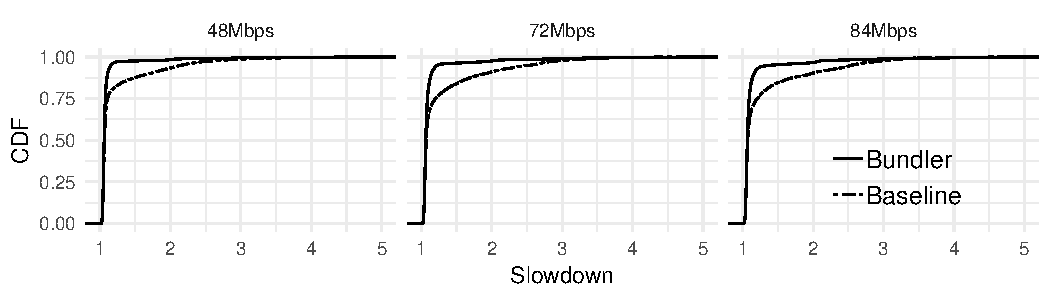
\includegraphics[width=\maxwidth]{figure/eval:offeredload-1} 

\end{knitrout}
    \caption{\name offers diminishing returns with lower amounts of offered load.}
    \label{fig:eval:offeredload}
\end{figure*}
%
%\newcommand{\highUtilTailImprove}{round(highUtilTailImprove, 0)\%\xspace}
%\newcommand{\medUtilTailImprove}{round(medUtilTailImprove, 0)\%\xspace}
%\newcommand{\lowUtilTailImprove}{round(lowUtilTailImprove, 0)\%\xspace}
